\chapter{Anwendung des Frameworks auf jadice flow}
\label{chap:anwendung}

In diesem Kapitel wird ein Architektur-Refactoring am Produkt \emph{jadice flow} geplant und in theoretischer Ebene durchgeführt.
Dazu werden \acrfull{mmf} und \acrfull{arh} verwendet, welche den Prozess sowie auch dieses Kapitel in drei Phasen unterteilen.
Eine genauere Beschreibung des Frameworks ist in \cref{sec:mmf} zu finden.
Sehr abstrahiert und vereinfacht bestehen die Phasen aus den folgenden Aktivitäten:
\begin{itemize}
	\item In \cref{sec:durchführung-phase1} wird die Durchführung der ersten Phase in Form eines Architekturreviews mit den wichtigsten Stakeholdern beschreiben.
	\item Im Rahmen der zweiten Phase wird in \cref{sec:durchführung-phase2} nach adäquaten Migrationsstrategien gesucht.
	\item In \cref{sec:durchführung-phase3} wird in der dritten Phase nach profitablen Patterns und Best Practices gesucht.
\end{itemize}

\section{Phase 1 - Systemverständnis}
\label{sec:durchführung-phase1}

Das Ziel dieser Phase ist es, ein Verständnis des Systems aufzubauen.
Das ist zum einen auf Seite der Stakeholder wichtig.
Diese sollten spätestens nach dieser Phase wissen, welche \acrfullpl{qa} besonders wichtig für das System sind.
Zum anderen sollte der \gls{arh} nach dieser Phase durch Eingabe der \glspl{qa} ein Verständnis des Systems erlangen, das er in den nächsten Phasen zur Unterstützung der Entwickler bei Migration verwenden kann.
Um das Systemverständnis zu erlangen, wurde in dieser Phase am 6. November 2023 ein Architekturreview wie in \cref{sec:methodik-architekturreview} beschrieben durchgeführt und am 14. November 2023 fortgesetzt.
Teilgenommen haben vier Softwareentwickler beziehungsweise -Architekten, der \acrlong{po} und der Autor selbst in der Rolle des Moderators.
Leider war es nicht möglich, einen Kunden oder Nutzer des Produkts als Stakeholder für dieses Review zu organisieren.
Da das Entwicklungsteam jedoch regelmäßigen Kontakt mit Kunden hat, haben sie bestmöglich versucht, auch die Interessen der Kunden zu repräsentieren.
Der Zeitrahmen für diese Besprechung war durch die Planung, die in \cref{sec:methodik-architekturreview} beschrieben ist, auf zwei Stunden festgelegt.
Im Folgenden wird der Begriff \emph{Schritt} immer auf den Schritt nach der beschriebenen Methodik bezogen und nicht auf Schritte des \gls{arh}.
Da der erste Schritt dabei lediglich eine Einführung in die Methodik ist, wird direkt mit den Ergebnissen des zweiten Schritts fortgefahren.

\subsection{Priorisierung der Qualitätsattribute (Schritt 2)}

Im zweiten Schritt werden die gewünschten \glspl{qa} des Systems gesammelt.
Im Rahmen dessen sollte jeder Teilnehmer seine Einschätzung darüber, welche die wichtigsten drei Sub-\glspl{qa} sind, per Nachricht mitteilen.
Die daraus resultierende Anzahl von Stimmen pro Sub-\gls{qa} ist in \cref{fig:qas-priority} dargestellt. 
% \begin{table}
  \centering
  \begin{tabular}{m{2.6cm} m{3.2cm} m{1.3cm} m{1.3cm}}
    \toprule
    \textbf{\gls{qa}} & \textbf{Sub-\gls{qa}} & \textbf{Anzahl Stimmen} & \textbf{Priorität} \\ \midrule
    Scalability & & 4 & 1\\ \hline

    \multirow{8}{=}[-0.1cm]{Maintainability} & Modularity & 4 & 2 \\
    & Monitorability & 2 & \\
    & Modifiabiltiy & 1 &  \\
    & Reusability & 1 &  \\
    & Testability & 1 &  \\
    & Analysability & 1 &  \\
    & Manageability & 1 &  \\
    & Understandability & 1 &  \\ \hline

    \multirow{2}{=}[-0.05cm]{Performance} & Time Behavior & 2 & 3 \\
    & Resource Utilization & 1 &  \\ \hline

   \multirow{5}{=}[-0.1cm]{Portability} & Deployability & 2 & 4 \\
   & Installability & 1 &  \\
   & Adaptability & 1 &  \\
   & Replaceability & 1 &  \\
   & Agility & 1 &  \\ \hline

    \multirow{3}{=}[-0cm]{Reliability} & Fault Tolerance & 1 & 5 \\
    & Recoverability & 1 & 6 \\
    & Availability & 1 &  \\ \hline

    Security & Confidentiality & 1 &  \\
    \bottomrule
  \end{tabular}
  \caption[Priorisierung der (Sub-) QAs durch Umfrage im Architekturreview]{
    Priorisierung der (Sub-) QAs durch Umfrage im Architekturreview in Phase 1 der Migration.
  }
  \label{tab:phase1-qas-priority}
\end{table}

\begin{figure}
	\centering
	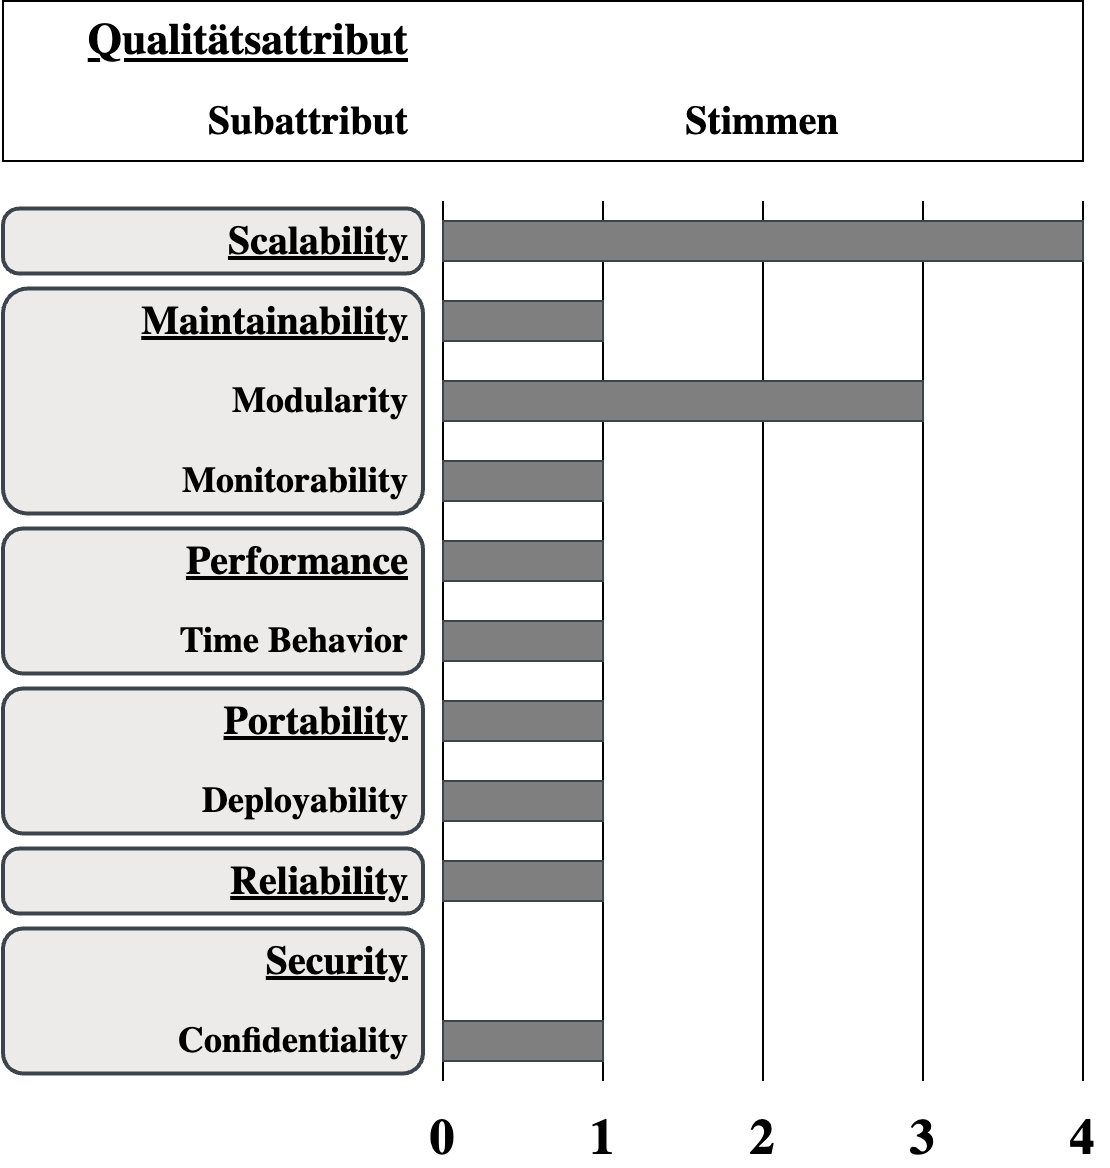
\includegraphics[width=0.8\textwidth]{qas-priority.drawio}
	\caption[Umfrageergebnisse wichtigste (Sub-) QAs im Architekturreview]{
		Umfrageergebnisse bei der Suche nach den wichtigsten (Sub-) QAs im Architekturreview in Phase 1 der Migration mit N = 5.
	}
	\label{fig:qas-priority}
\end{figure}
Dabei ist auffällig, dass auch  \acrlongpl{qa} Stimmen erhalten haben.
Das liegt daran, dass nicht alle Teilnehmer der Umfrage sich auf Sub-\glspl{qa} beschränkt haben, sondern auch die \glspl{qa} \emph{Performance}, \emph{Reliability}, \emph{Maintainability} und \emph{Portability} genannt wurden.
Auch wenn das nicht so vorgesehen war, wurde davon abgesehen, die Teilnehmer darauf hinzuweisen und es zu korrigieren, da die Ergebnisse nicht direkt zur Priorisierung der Attribute führen müssen.
Stattdessen wurden die Umfrageergebnisse und als vage Basis für eine freiere Diskussion über die Priorisierung verwendet. 
Deren Ergebnis war die schlussendliche Platzierung der sechs wichtigsten Sub-\glspl{qa}.
Im Folgenden werden diese erläutert.
\begin{enumerate}
	\item \textbf{\emph{Scalability}} ist ein \gls{qa} ohne Subattribute, es wird allerdings auch oft \emph{Performance} zugeordnet. Nach \Citet{master-daniel-koch} gibt es an, wie effizient ein System skaliert werden kann~\cite{koch-scalability-1}. Im Kontext von Microservices ist dabei vor allem die horizontale Skalierung relevant, welche die Skalierung über mehrere Instanzen von der Microservices beschreibt~\cite{koch-scalability-2}.
	\item \textbf{\emph{Modularity}} ist ein Subattribut von \emph{Maintainability}. Nach \Citet{master-daniel-koch} gibt es an, wie gut die Komplexität des Systems auf verschiedene Komponenten verteilt ist~\cite{ISO-25010}.
	\item \textbf{\emph{Time Behavior}} ist Subattribut von \emph{Performance}. Nach \Citet{master-daniel-koch} gibt es an, wie schnell ein System oder Teile eines Systems ankommende Anfragen beantworten~\cite{ISO-25010,koch-time-behavior-1,koch-time-behavior-2}.
	\item \textbf{\emph{Deployability}} ist ein Subattribut von \emph{Portability}. Nach \Citet{master-daniel-koch} gibt es an, wie einfach und schnell ein Produkt gebaut und ausgeliefert werden kann~\cite{koch-scalability-1,koch-deployability}.
	\item \textbf{\emph{Fault Tolerance}} ist Subattribut von \emph{Reliability}. Nach \Citet{master-daniel-koch} gibt es an, inwieweit ein System wie erwartet funktionieren kann, obwohl in Teilen des Systems Fehler passieren~\cite{ISO-25010,koch-fault-tolerance}.
	\item \textbf{\emph{Recoverability}} ist ebefalls Subattribut von \emph{Reliability}. Nach \Citet{master-daniel-koch} gibt es an, inwieweit ein System nach einem Ausfall wieder den Zustand vor dem Ausfall herstellen kann, sowie Daten erhalten kann~\cite{ISO-25010}.
\end{enumerate}
Die genaue Anzahl der wichtigsten (Sub-)Attribute war nicht vor dem Termin definiert, sondern wurde ebenfalls von der Gruppe diskutiert (in einem späteren Schritt) und gemeinsam auf sechs festgelegt.
Der gesamte Prozess der Umfrage und anschließender Diskussion, um die Prioritäten der Attribute zu setzen, dauerte etwa 15 Minuten und entsprach somit der geplanten Zeit.

\subsection{Szenarienerhebung (Schritt 3)}

Im nächsten Schritt war die Aufgabe, für jedes dieser (Sub-) \glspl{qa} zwei Szenarien zu definieren, die das Attribut gut und auf verschiedene Arten beschreiben.
Es wurde keine spezielle Methodik angewandt, sondern in einer offenen Diskussion der gesamten Gruppe von verschiedenen Teilnehmern nacheinander für die Attribute Szenarien vorgeschlagen und anschließend überarbeitet oder teilweise auch abgelehnt.
Diese Szenarien wurden in Form eines \emph{Utility Trees}, beschrieben in \cref{sec:atam-saam-svahnberg}, festgehalten.
Nach einer Diskussionszeit von etwa 35 Minuten ergaben sich die Szenarien, die in  \cref{fig:scenarios} abgebildet sind. 

\begin{figure}
	\centering
	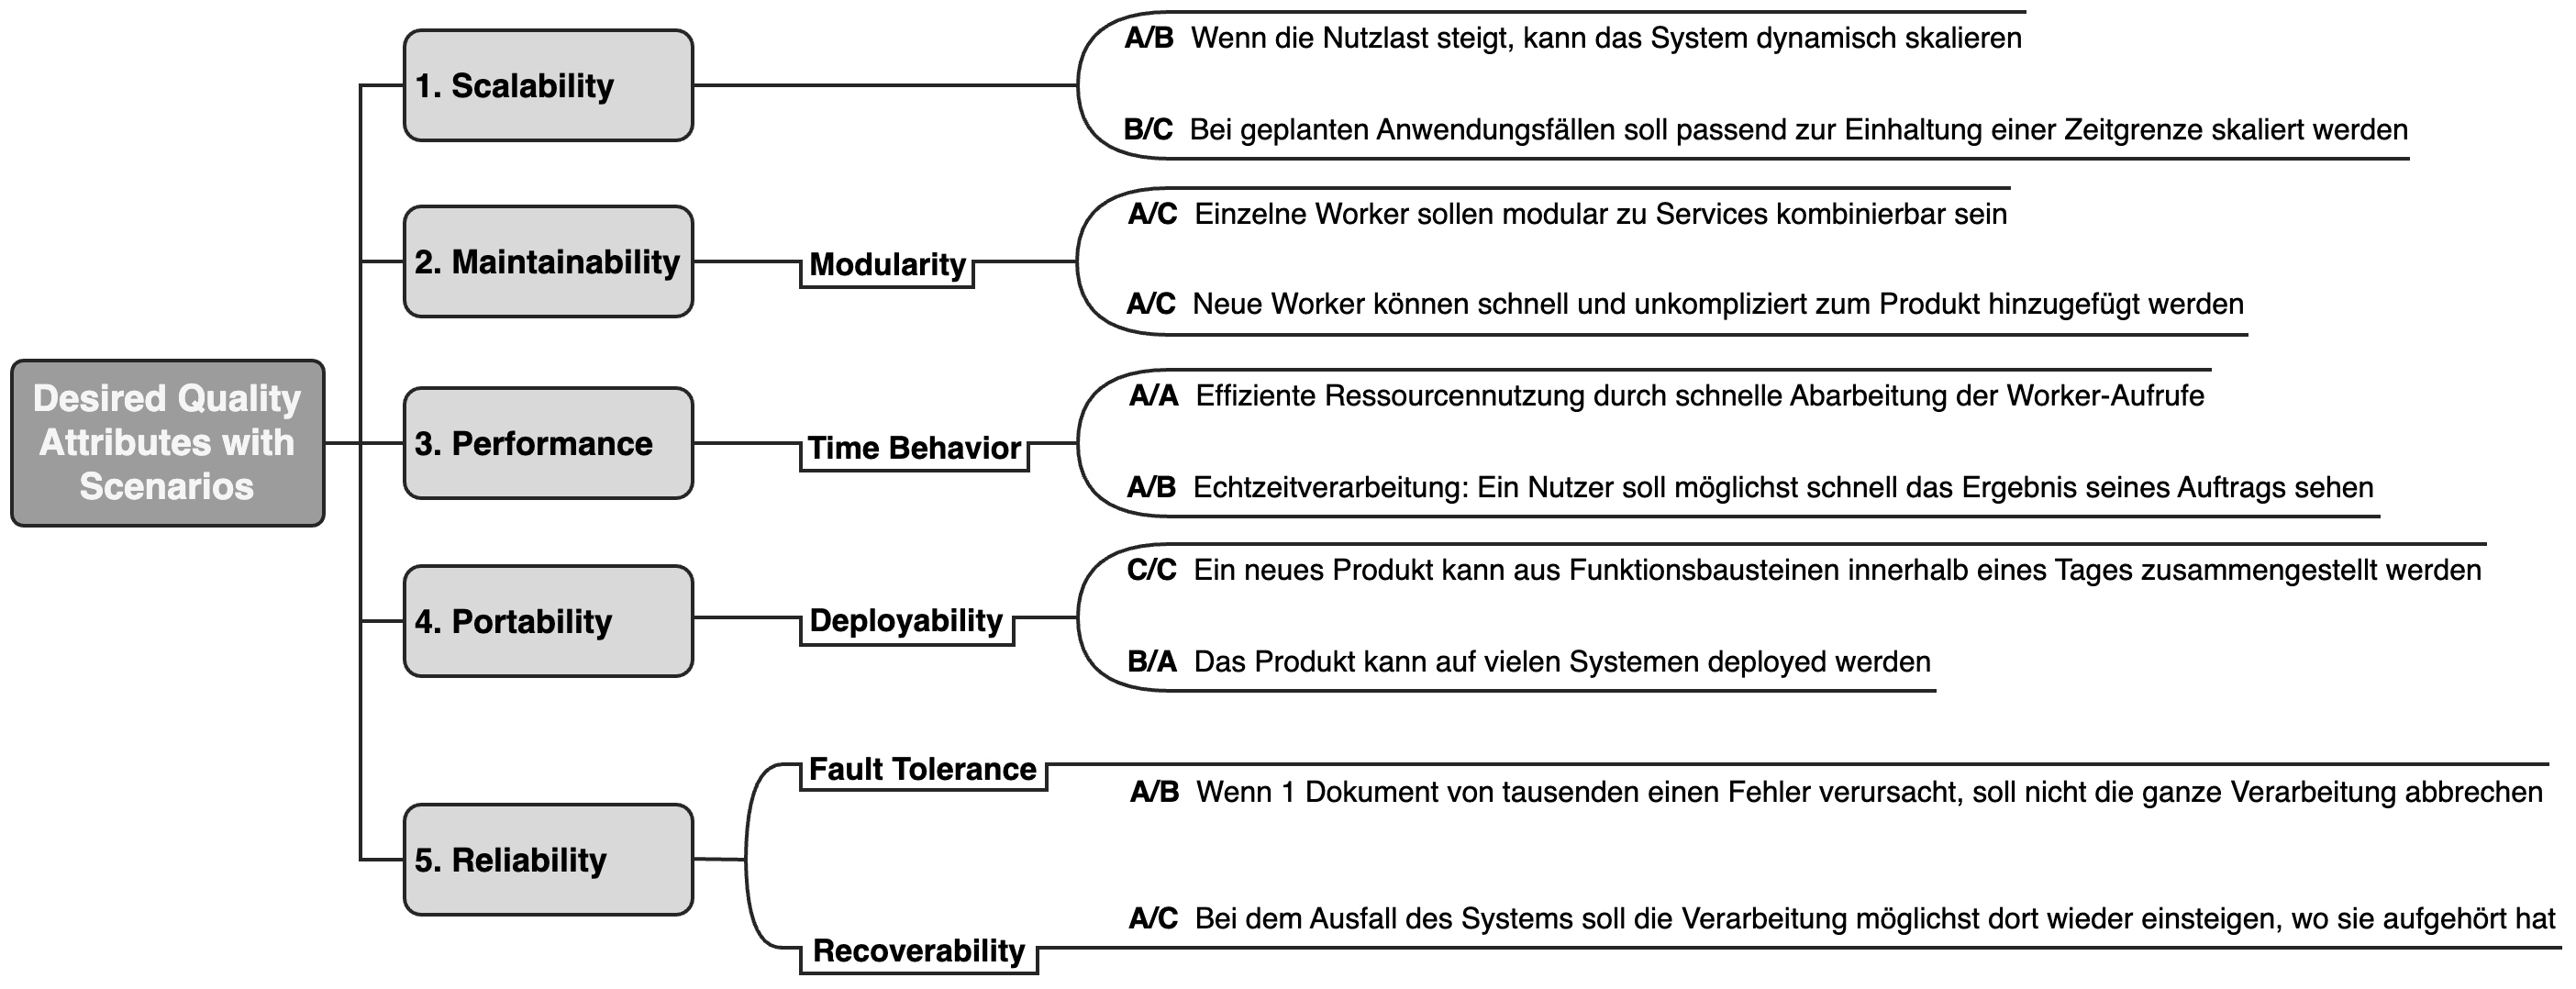
\includegraphics[angle=270,width=\textwidth]{scenarios.drawio}
	\caption[Utility Tree mit im Architekturreview ermittelten Qualitätsanforderungen und Szenarien]{
		Der Utility Tree mit Szenarien, die aus dem in Phase 1 durchgeführten Architekturreview resultieren.
		Von oben nach unten enthält der Baum folgende Elementarten: [1] Wurzel (ohne Bedeutung), [2] \gls{qa}, [3] Subattribut, [4] Beurteilung des Szenarios hinsichtlich Wichtigkeit und technischer Schwierigkeit, [5] Szenariobeschreibung.
	}
	\label{fig:scenarios}
\end{figure}

Wie aus der Abbildung ersichtlich, wurden für jedes (Sub-)Attribut mit Ausnahme von \emph{Fault Tolerance} und \emph{Recoverability} jeweils zwei Szenarien erstellt.
Dies hat zwei Gründe.
Zum einen wurden für diese Subattribute keine ausreichend unterschiedlichen Szenarien gefunden. 
Zum anderen wurde in diesem Fall ein Szenario als ausreichend betrachtet, da Reliability das einzige QA ist, für das mehrere Subattribute eingeschlossen wurden. 
Darüber hinaus ist es das am geringsten priorisierte Attribut.

Um zusätzliche eine Priorisierung der Szenarien vornehmen zu können, sieht der \gls{arh} jeweils eine dreistufige Bewertung der Szenarien hinsichtlich ihrer Wichtigkeit und ihrer technischen Schwierigkeit vor.
Diese wurde im nächsten Schritt vorgenommen.
Dabei haben die Teilnehmer die Szenarien der Reihe nach betrachtet und ihre Wichtigkeit und technische Schwierigkeit diskutiert.
Nicht immer waren alle anfangs einer Meinung, doch schlussendlich konnte nach etwa 35 Minuten für jedes Szenario Konsens gefunden werden und diese Phase abgeschlossen werden.

Da die Vollendung des dritten Schritts nach \Citet{SVAHNBERG20071893} länger gedauert hat als geplant, waren am Ende dieses Termins nur noch wenige Minuten übrig.  
Für alle Sub-Schritte dieses Schritts zusammen waren nur 60 Minuten eingeplant, das Sammeln der Szenarien und das Bewerten dieser (also zwei von drei Sub-Schritten) nahm jedoch schon 70 Minuten in Anspruch.
Daher wurde entschieden, die restlichen Punkte in einer weiteren Sitzung in der nächsten Woche zu bearbeiten.

Am 14. November 2023 wurde dann der zweite Teil des Architekturreviews durchgeführt.
Anwesend waren dieselben Personen.
Da bei diesem Treffen ein neuer Blickwinkel auf die Thematik möglich gewesen wäre, wurden zunächst zehn Minuten darauf verwendet, die bereits vorhandenen Szenarien und die Bewertung dieser hinsichtlich Wichtigkeit oder technischer Schwierigkeit erneut zu überprüfen und Raum für mögliche Änderungen zu schaffen.
Es wurden jedoch keine Änderungen vorgenommen und die Teilnehmer bestätigten lediglich erneut die bereits vorhandenen Szenarien.

Anschließend wurde wie geplant damit fortgefahren, den Szenarien weitere \glspl{qa} zuzuordnen.
Oft können trotz der Erstellung eines Szenarios für ein bestimmtes \gls{qa} weitere \glspl{qa} damit assoziiert werden.
Deswegen wurde erneut jedes Szenario betrachtet und diskutiert, welche weiteren (Sub-) Attribute darauf zutreffen könnten.
Nach etwa 15 Minuten Diskussion waren alle Szenarien behandelt und für jedes einstimmig geklärt, welche weiteren Subattribute damit assoziiert werden.
Diese werden folgend im Bezug auf die jeweiligen Szenarios sekundäre \glspl{qa} genannt, wohingegen ein \gls{qa}, für das das Szenario erstellt wurde, primäres \gls{qa} genannt wird.
Die resultierenden Assoziationen sind in der \cref{tab:scenarios} aufgeführt.

\begin{table}[!h]
  \centering
  \begin{tabular}{ m{2,3cm} m{6cm} m{0.7cm} m{2,5cm} p{0.7cm} }
    \toprule
    \textbf{Name} & \textbf{Beschreibung} & \textbf{W/S} & \textbf{\glspl{qa}} & \textbf{MS} \\
    \midrule
    Dynamische Ska\-lier\-bar\-keit & Wenn die Nutzlast steigt, kann das Sys\-tem dynamisch skalieren & A/B & Scalability, Re\-source Uti\-li\-za\-tion, Adaptability, Execution Cost & \advantage \\ \hline
    Statische Ska\-lier\-bar\-keit & Bei geplanten Anwendungsfällen soll passend zur Einhaltung einer Zeitgrenze skaliert werden & B/C & Scalability, Resource Utilization, Time Behavior & \advantage \\  \hline
    Jobtemplates& Einzelne Worker sollen modular zu Services kombinierbar sein & A/C & Modularity, Reusability & - \\ \hline
    Neue Worker& Neue Worker können schnell und un\-kom\-pliziert zum Produkt hinzugefügt werden & A/C & Modularity, Reusability & \advantage  \\ \hline
    Schnelle Ab\-ar\-bei\-tung & Effiziente Ressourcennutzung durch schnelle Abarbeitung der Worker-Auf\-rufe  & A/A & Time Behavior, Resource Uti\-li\-za\-tion & \disadvantage \\ \hline
    \glqq Echtzeit\grqq{}-Verarbeitung & Ein Nutzer soll möglichst schnell das Ergebnis seines Auftrags sehen & A/B & Time Behavior & \disadvantage \\ \hline
    Einfaches De\-ploy\-ment & Ein neues Produkt kann aus Funk\-tions\-bausteinen innerhalb eines Tages zusammengestellt werden &C/C & Deployability, Modularity, Agility & \disadvantage \\ \hline
    Platform-unabhängigkeit& Das Produkt kann auf vielen Systemen deployed werden & B/A & Deployability, Installability & \advantage \\ \hline
    Fehlerto\-leranz Massen\-ver\-ar\-beitung & Wenn 1 Dokument von tausenden einen Fehler verursacht, soll nicht die ganze Verarbeitung abbrechen & A/B & Fault-Tolerance &\advantage \\ \hline
    Erholen nach Sys\-tem\-ausfall & Bei dem Ausfall des Systems soll die Verarbeitung möglichst dort wieder einsteigen, wo sie aufgehört hat & A/C & Recoverability & - \\
    \bottomrule
  \end{tabular}
  \caption[Im Architekturreview ermittelte Qualitätsanforderungen und Szenarien]{
    Szenarien, die aus dem in Phase 1 durchgeführten Architekturreview resultieren.
    \emph{W/S} gibt die Wichtigkeit/Schwierigkeit der Szenarien in drei Stufen an (A steht für sehr wichtig und sehr schwierig).
    \emph{\glspl{qa}} gibt die Assoziation der Szenarien zu bestimmten \acrfullpl{qa} an; zuerst genannte sind primäre \glspl{qa}, folgende sekundäre \glspl{qa}.
    \emph{MS} gibt die Einschätzung darüber an, ob das jeweilige Szenario von einer Microservices-Architektur profitiert.
  }
  \label{tab:scenarios}
\end{table}


Damit wurde der für die Extraktion der Qualitätsanforderungen des Systems relevante Teil des Architekturreviews abgeschlossen.
Zusammenfassend kann gesagt werden, dass die Phase größtenteils wie geplant durchgeführt werden konnte.
An einigen Stellen sind die verschiedene Schritte etwas verschmolzen oder es wurde kurz zu vorherigen Schritten zurückgesprungen, was jedoch vollkommen normal ist und auch beispielsweise in \gls{atam} von \Citet{kazman_2000} als gängige Praxis beschrieben wird.
So wurde in diesem Fall beim Erstellen der Szenarien entschieden, bis zu welcher Priorität die \glspl{qa} mit Szenarien versehen werden, obwohl die Wahl der Anzahl der wichtigsten tatsächlich für den vorherigen Schritt geplant war.
Die Beteiligung der Teilnehmer war komplett ausgeglichen, aber jeder hat regelmäßig etwas beigetragen.
Es kann angenommen werden, dass das Ergebnis von allen Teilnehmern ausreichend geformt wurde und dass keine einseitige Beeinflussung vorliegt.

\subsection{Architekturanalyse anhand Szenarien (Schritt 5)}

Neben der Erfassung der wichtigsten Szenarien und \glspl{qa} hatte die Fokusgruppe als sekundäres Ziel, die Wahl der Architektur für \emph{jadice flow} zu bewerten. 
Diese Bewertung wurde ebenfalls in der zweiten Sitzung des Architekturreviews durchgeführt und entspricht dem vierten Schritt \emph{Assessment} der ersten Phase des \gls{arh}.
Da dieser Schritt jedoch noch nicht im Werkzeug implementiert ist, wurde er manuell durchgeführt.
Im Gegensatz zu vorherigen Schritten der ersten Phase ist dieser nicht relevant für die nächsten Phasen, weshalb es kein Problem ist, den \gls{arh} hierbei nicht zu verwenden.
In diesem Schritt wurde die Frage diskutiert, ob eine \acrlong{msa} individuell für jedes Szenario vorteilhaft ist im Vergleich zu einer monolithischen Architektur.
Hierbei wurde in drei Stufen unterschieden:
\begin{itemize}
	\item \advantage\hspace*{0.1cm}: Dieses Szenario profitiert wesentlich mehr von einer \gls{msa} als von einer monolithischen Architektur.
	\item \disadvantage\hspace*{0.1cm}: Dieses Szenario profitiert wesentlich mehr von einer monolithischen Architektur als von einer \gls{msa}.
	\item \hspace*{0.27cm}-\hspace*{0.27cm}: Dieses Szenario profitiert in verschiedenen Punkten sowohl von einer \gls{msa} als auch von einer monolithischen Architektur, wobei sich beide Seiten ungefähr gleichen.
\end{itemize}
Bei Szenarios wie beispielsweise den des \emph{Scalability} Attributs war es nicht schwer, Konsens zu finden, da die Möglichkeit der Skalierung auf Service-Ebene einer der größten Vorteile von \glspl{msa} gegenüber Monolithen ist.
In anderen Fällen jedoch war es schwieriger, abzuwägen, ob die Vorteile einer \gls{msa} oder die eines Monolithen überwiegen.
Schlussendlich konnte jedoch in Form von offener  Diskussion für jedes Szenario einstimmig geklärt werden, welche der drei Optionen gewählt werden sollte, sodass keine Abstimmungen notwendig waren.

Das Ergebnis dieser Einschätzungen ist ebenfalls in \cref{tab:scenarios} zu sehen.
Insgesamt wurde eine \gls{msa} in fünf Fällen als vorteilhaft und nur in drei Fällen als unvorteilhaft bewertet. 
Des Weiteren ist zu beachten, dass die Szenarien in der Tabelle nach der Wichtigkeit der primären \glspl{qa} sortiert sind und die obersten beiden Szenarien die Hauptfaktoren für die Migration zu einer Microservices-Architektur waren.
Durch die Überlegenheit der \gls{msa}-Favorisierungen und dass diese verstärkt bei den wichtigsten \glspl{qa} vorliegen, kann diese Auswertung die Entscheidung zur Migration zu einer \gls{msa} bestätigen.

Nachdem nun erwünschte Szenarien und \glspl{qa} erhoben wurden und die Wahl einer \gls{msa} für \emph{jadice flow} bekräftigt wurde, kann mit Phase 2 fortgefahren werden.

\section{Phase 2 - Strategieplanung}
\label{sec:durchführung-phase2}

In dieser Phase werden die Ergebnisse der Phase 1 in Form von \glspl{qa} beziehungsweise Szenarien genutzt, um eine passende Migrationsstrategie zu finden.
Dazu wurden die in \cref{tab:scenarios} dargestellten Szenarien bereits in den \gls{arh} eingegeben.
Zusätzlich werden in dieser Phase Filterkriterien definiert.
Mit deren Hilfe wird dann schlussendlich eine Liste von Migrationsstrategien vorgeschlagen, welche folgend analysiert wird.

\subsection{Filterselektion}
\label{sec:filterselektion}
Damit bei der Suche nach Migrationsmethoden möglichst gut zum Zielsystem und den Vorstellungen der Architekten passende Ergebnisse vorgeschlagen werden, bietet der \gls{arh} neben der Konfiguration der Szenarien noch eine weitere Art, die Ergebnisse zu filtern und ordnen: Die Filter, die in diesem Abschnitt konfiguriert werden.
Dabei kann für jede der Eigenschaften aus \cref{tab:phase2-filter} eine dieser drei Präferenzen angegeben werden:
\begin{itemize}
	\item \textbf{Include:} Methoden, die die jeweilige Eigenschaft haben, werden höher platziert.
	\item \textbf{Neutral:} Ob Methoden die jeweilige Eigenschaft haben, wirkt sich nicht auf ihre Platzierung aus.
	\item \textbf{Exclude:} Methoden, die die jeweilige Eigenschaft nicht haben, werden höher platziert.
\end{itemize}
Dabei wird es in den meisten Fällen zielführender sein, präferierte Eigenschaften auf \emph{include} zu setzen und die anderen bei der Standardeinstellung \emph{neutral} zu belassen und die Einstellung \emph{exclude} nicht zu verwenden, da nur selten das Ziel sein dürfte, eine bestimmte Eigenschaft auszuschließen.

\begin{table}
  \centering
  \begin{tabular}{m{2cm} m{2cm} m{9cm}}
    \toprule
    \textbf{Kategorie} & \textbf{Subkategorie} & \textbf{Eigenschaften} \\
    \midrule
    Quality Preferences & System Properties & Autonomy, Cohesion, Complexity, Coupling, Granularity, Isolation, Technology Heterogenity \\ \hline
    \multirow{4}{=}[-1cm]{Input Preferences} & Domain Artifacts &  Documentation, Human expertise, Ontology, Version Control System \\ \cline{2-3}
    & Runtime artifacts & Log traces, User-Application interactions \\ \cline{2-3}
    & Model artifacts & Activity diagram, Business process model, Class diagram, Custom model, Data flow diagram, Entity model, State machine diagram, Use case model \\ \cline{2-3}
    & Executables & API / Interface, Database file, Source code (Java), Source code (No specification), Source code (Python), Test cases \\ \hline
    \multirow{6}{=}[-1.9cm]{Process Preferences} & Directions & Bottom-up, Mixed, Top-down \\ \cline{2-3}
    & Levels of automation & Automatic, Manual, Semi-automatic \\ \cline{2-3}
    & Analysis types & Dynamic, Historic, Lexical, Static \\ \cline{2-3}
    & Techniques & Clustering, Custom heuristics, Data-flow driven, Domain-Driven Design, Execution-trace modeling, General guidelines, Genetic algorithm, Graph-based, Machine Learning, Multi-Tenancy, Performance modeling, Scenario analysis, Wrapping / Black Box \\ \cline{2-3}
    & Process Strategy & Continuous Evolution, Extension, Greenfield, Refactor, Rewrite / Rebuild, Strangler \\ \cline{2-3}
    & Atomar Unit & Business Capability, Class, Entity, Function, Functionality, Interface, Other \\ \hline
    Output Preferences & Representation & Guideline / Workflow, List of services, Source code, Splitting recommendations, Visualization \\ \hline
    \multirow{4}{=}[-1cm]{Usability Preferences} &Validation methods & Case study, Experiment, Industry, No validation \\ \cline{2-3}
    & Accuracy of \gls{sia} & High, Medium, Low, Not available \\ \cline{2-3}
    & Tool supports &  No tool support \\ \cline{2-3}
    & Tool types & Database, Decomposition, Dynamic Analysis, Java, Open Source, Other, Reverse Engineering, Static Analysis, Visualization \\
    \bottomrule
  \end{tabular}
  \caption[Mögliche Filter des \gls{arh} in Phase 2]{
    Mögliche Filter des \gls{arh} in Phase 2.
  }
  \label{tab:phase2-filter}
\end{table}


Für die Wahl der Filter für das Refactoring von \emph{jadice flow} haben \gls{po} und der Autor alle Filter betrachtet und die wichtigsten relevanten ausgewählt (\cref{feldnotiz:1,feldnotiz:2}).
Diese sind \cref{tab:phase2-filter} markiert.
Dabei wurden die \glspl{sp} als am wichtigsten betrachtet, weswegen dort viele Eigenschaften inkludiert wurden.
Bei den anderen Kategorien wurde versucht, nur die wichtigsten Filter zu verwenden, da mit zu vielen Filtern eine geringere Aussagekraft dieser vermutet wird.
Vor allem \emph{Process Preferences} und \emph{Usability Preferences}, also Eigenschaften, die die interne Funktionsweise der Methode betreffen, wurden als relativ unwichtig und vor allem auch unabhängig vom betreffenden System eingestuft und demnach nur ein einziger dieser Filter verwendet.
Dieser betrifft die \emph{Process Strategy}, wobei \emph{Refactoring} ausgewählt wurde, da bereits eine \gls{msa} vorliegt und somit Optionen wie \emph{Rewrite/Rebuild} wenig sinnvoll wären.
Am wichtigsten neben den \glspl{sp} wurden \emph{Input Preferences} und \emph{Output Preferences} eingestuft, da diese ebenfalls stark vom System abhängen und Ausgangslage und gewünschtes Ergebnis betreffen.

Wie ebenfalls in \cref{tab:phase2-filter} ersichtlich ist, wurden die ausgewählten Filter in zwei Prioritäten unterteilt (\cref{feldnotiz:3}).
Das soll dem Ziel dienen, mit mehreren Einstellungen der Filter Suchen durchführen zu können: 
Eine Suche wird mit allen Filtern stattfinden und eine Suche nur die höher priorisierten Filter beinhalten.
Dadurch sollen auf der einen Seite bessere Ergebnisse erzielt werden und auf der anderen Seite die Filterfunktion untersucht werden.
Die Ergebnisse dessen werden im Folgenden besprochen.

\subsection{Suchergebnisbetrachtung}
\label{sec:phase2-ergebnisdurchsicht}

Die Filter, die im vorherigen Abschnitt gewählt wurden, werden in diesem Abschnitt angewendet, um jeweils geordnete Listen von Ergebnissen zu erhalten.
In \cref{tab:phase2-filter-results} sind die jeweils ersten fünf Ergebnisse der Suchen mit allen Filtern, mit den wichtigsten Filtern und ohne zusätzliche Filter, nur mit dem \glspl{qa} zu sehen. 

\begin{table}[!ht]
	\centering
	\begin{tabular}{l c c c}
		\toprule
    \textbf{Publikation} & \multicolumn{3}{c}{\textbf{Matches}} \\
     & \textbf{Insgesamt} & \textbf{\gls{qa}} & \textbf{\gls{sp}} \\ \midrule
    \multicolumn{4}{c}{\textbf{Alle Filter (15)}} \\ \midrule
    \Citet{arh-result-no-filter-1} & 15/32 & 11/17 & 0/5 \\ \hline
    \Citet{arh-result-no-filter-3} & 13/32 & 7/17  & 1/5  \\ \hline
    \Citet{arh-result-no-filter-2} & 12/32 & 7/17  & 2/5  \\ \hline
    \Citet{arh-result-no-filter-4} & 11/32 & 7/17  & 0/5  \\ \hline
    \Citet{arh-result-no-filter-5} & 11/32 & 7/17  & 0/5  \\ \midrule
		\multicolumn{4}{c}{\textbf{Wichtigste Filter (9)}} \\ \midrule
		\Citet{arh-result-no-filter-1}        & 14/26 & 11/17 & 0/3 \\ \hline
		\Citet{arh-result-no-filter-3}        & 13/26 & 7/17  & 1/3  \\ \hline
		\Citet{arh-result-no-filter-2}        & 11/26 & 7/17  & 1/3  \\ \hline
		\Citet{arh-result-important-filter-4} & 10/26 & 6/17  & 1/3  \\ \hline
    \Citet{arh-result-no-filter-4}        & 10/26 & 7/17  & 0/3  \\ \hline
    \textbf{\Citet{arh-result-no-filter-5}}        & 10/26 & 7/17  & 0/3  \\ \hline
    \textbf{\Citet{arh-result-important-filter-7}}        & 10/26 & 5/17  & 1/3  \\ \midrule
    \multicolumn{4}{c}{\textbf{Keine Filter (Nur \glspl{qa})}} \\ \midrule
    \Citet{arh-result-no-filter-1} & 11/17 & 11/17 & - \\ \hline
    \Citet{arh-result-no-filter-2} & 7/17  & 7/17  & - \\ \hline
    \Citet{arh-result-no-filter-3} & 7/17  & 7/17  & - \\ \hline
    \Citet{arh-result-no-filter-4} & 7/17  & 7/17  & - \\ \hline
    \Citet{arh-result-no-filter-5} & 7/17  & 7/17  & - \\ \bottomrule
	\end{tabular}
	\caption[Surchergebnisse des ARH von Migrationsverfahren mit verschiedenen Filtern]{
		Ergebnisse der Suche mit ARH nach Migrationsverfahren mit verschiedenen Filtern, wie in \cref{sec:filterselektion} näher beschrieben, nach Matches sortiert.
		Insgesamte Matches, \gls{sp} Matches und \gls{qa} Matches entsprechen den im \gls{arh} angezeigten Matches.
	}
	\label{tab:phase2-filter-results}
\end{table}


Um einen Gesamtvergleich über alle Suchen zu erhalten, sind die Ergebnisse in Tabelle \cref{tab:phase2-ranking} nach prozentualer Übereinstimmung mit der Suche platziert.
\begin{table}[!h]
  \centering
  \begin{tabular}{m{2cm} m{4.3cm} m{4.3cm} m{2.5cm}}
    \toprule
    \textbf{Ergebnis} & \textbf{Matches Prozent ($m_{gesamt}$)} & \textbf{Manuelle Bewertung} & \textbf{Kommentare} \\ \midrule
    \cite{arh-result-no-filter-1} & $53,9\%$ & & \\ \hline
    \cite{arh-result-no-filter-3} & $44,9\%$& & \\ \hline
    \cite{arh-result-no-filter-2} & $40,5\%$& & \\ \hline
    \cite{arh-result-no-filter-4} & $37,7\%$& & \\ \hline
    \cite{arh-result-no-filter-5} & $37,7\%$& & \\ \hline
    \cite{arh-result-important-filter-4} & $35,4\%$& & \\
    \bottomrule
  \end{tabular}
  \caption[Platzierung der Suchergebnisse in Phase 2 des \gls{mmf}]{
   	Platzierung der Suchergebnisse in Phase 2 des \gls{mmf}.
  }
  \label{tab:phase2-ranking}
\end{table}

Diese setzt sich zusammen aus:
\[
m_{gesamt} = \frac{2 \cdot m_{Wichtigste \text{ } Filter} + 1,5 \cdot  m_{Alle \text{ } Filter} +  m_{Keine \text{ } Filter}}{4,5}
\]
wobei $m_{gesamt}$ die gesamte prozentuale Übereinstimmung darstellt, also das Ergebnis, das in \cref{tab:phase2-ranking} angezeigt wird.
$m_{Wichtigste \text{ } Filter}$, $m_{Alle \text{ } Filter}$ und $m_{Keine \text{ } Filter}$ sind dabei die prozentualen Matches, die in \cref{tab:phase2-filter-results} vorne stehen.
Das wären beispielsweise im Fall \Citet{arh-result-no-filter-1} $m_{Wichtigste \text{ } Filter} = \frac{14}{26} \approx 53,8\%$.
Es wurde eine Gewichtung gewählt, sodass die Matches des wichtigsten Filter doppelt so stark und die aller Filter 1,5-fach gewichtet werden wie die Matches ohne Filter.
Das ist damit zu begründen, dass die Filter mit der höchsten Gewichtung die realistischste Eingabe abbilden und damit relevanter sind.

\subsubsection{Ergebnis 1: \citetitle{arh-result-no-filter-1}  \cite{arh-result-no-filter-1}}

In dieser Arbeit wird konzeptuelles Evolutions-Framework vorgestellt, das mithilfe von Trans\-for\-ma\-tions\-re\-geln die Migration von Legacy-Systemen zu Microservices unterstützen soll.
Dabei ist das Vorgehen 
%wie in \cref{fig:arh-result-1} zu sehen 
in 3 Teilabschnitte unterteilt.
% TODO get copyright for this
%\begin{figure}[!h]
%	\centering
%	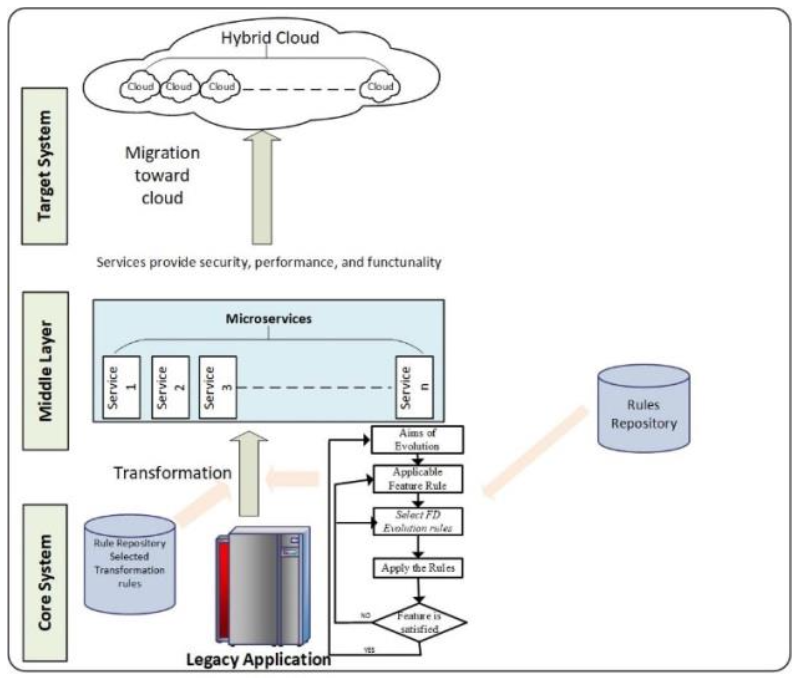
\includegraphics[width=0.7\textwidth]{arh-result-1}
%	\caption[Konzeptuelles Framework von \Citet{arh-result-no-filter-1}]{
%		Konzeptuelles Framework von \Citet{arh-result-no-filter-1}.
%	}
%	\label{fig:arh-result-1}
%\end{figure}
Das \emph{Core System} besteht aus dem Legacy System und einer Auswahl von Transformationsregeln.
Diese können aus der Sammlung von vorgestellten Regeln der Autoren stammen, aber auch durch eigene ergänzt werden.
Daraus erstellt man dann ein \emph{Middle Layer}, indem diese Tranformationsregeln auf das Legacy-System angewendet werden.
Daraus resultiert eine Dekomposition des Systems in Microservices.
Das \emph{Target System} kann dann entwickelt werden, indem die erhaltenen Services in einer hybriden Cloud, bestehend aus einer privaten und einer öffentlichen Cloud, umgesetzt werden.

Diese Vorgehensweise wurde auch in einer Fallstudie überprüft.
Bei dieser wurde ein öffentliches GitHub Projekt als Legacy System verwendet, welches dann mit drei der vorgestellten Transformationsregeln zu einer \gls{msa} migriert wurde.
Durch die Architekturänderung konnte das \emph{Coupling} reduziert werden, sowie die Modularität, Skalierbarkeit und Anfragezeit verbessert werden.
Jedoch sind diese Ergebnisse nur bedingt aussagekräftig und müssen auch laut den Autoren noch an mittel bis großen Industriesystemen reproduziert werden.

Insgesamt wirkt die Methode sehr abstrakt und oberflächlich und wenig spezifisch.

\subsubsection{Ergebnis 2: \citetitle{arh-result-no-filter-3} \cite{arh-result-no-filter-3}}

In diesem Artikel stellen die Autoren eine Methode vor, die sie anhand der ebenfalls durchgeführten Fallstudie mit Barcelonas Fahrradvermietung-System \emph{Bicing} erklären und validieren.
Sie besteht aus drei übergeordneten Schritten.
Im ersten Schritt werden die Eingaben für die Methode in Form von \glspl{bp} gesammelt und logisch verbunden, beispielsweise in Form eines \gls{bpmn}-Diagramms.
Für die Bestandteile dieser Eingabe (genannt Aktivitäten) werden dann im zweiten Schritt Abhängigkeiten in drei verschiedenen Formen analysiert.
Dabei handelt es sich um \emph{control dependencies}, \emph{data dependencies} und \emph{semantic dependencies}.
Eine \emph{control dependency} beschreibt eine Abhängigkeit zweier Aktivitäten im Kontrollfluss, also dass eine der Aktivitäten mit hoher Wahrscheinlichkeit auf die andere folgt.
Eine \emph{data dependency} beschreibt eine Abhängigkeit der Ein- oder Ausgaben zweier Aktivitäten, also einen Datenfluss zwischen den Aktivitäten.
Eine \emph{semantic dependency} beschreibt eine Ähnlichkeit des Zwecks zweier Aktivitäten. 
Die Messung solcher Abhängigkeiten kann aufgrund der Ähnlichkeit der Namen der Aktivitäten geschehen.

Im letzten Schritt wird die \emph{Machine Learning} Technik \emph{Collaborative clustering} verwendet, um die Menge von Aktivitäten in Gruppen (genannt \emph{Cluster}) zu unterteilen.
Die Autoren haben dazu den \gls{hac}~\cite{hierarchical-agglomerative-algorithm} erweitert.
Das Ziel ist dabei, dass Aktivitäten in einem Cluster hohe Kohäsion aufweisen und Aktivitäten verschiedener Cluster lose gekoppelt sind, sodass aus den Clustern potentiell Microservices entstehen können.

% TODO Einfügen der Übersicht: TODO get license: https://www.sciencedirect.com/science/article/pii/S1383762121001442?via%3Dihub

\subsubsection{Ergebnis 3: \citetitle{arh-result-no-filter-2} \cite{arh-result-no-filter-2}}

Dieser Artikel beschreibt die Methode \gls{mb}, ein semiautomatisches Modell zur Bewertung der Granularität einer \gls{msa}.
In Kontrast zu den meisten anderen Methoden, die im Rahmen dieser Thesis erwähnt werden, liegt hier also nicht der Kontext einer Migration, sondern eines Refactorings vor, was gut zu dieser Fallstudie mit \emph{jadice flow} passt.
Als Eingabe werden dabei \emph{User Stories} aus dem \emph{Product Backlog} oder der Release-Planung verwendet.
Diese werden in Kombination mit den Metriken \emph{Coupling}, \emph{Kohäsion}, \emph{Granularität}, \emph{semantische Ähnlichkeit} und \emph{Komplexität} von einem \emph{genetic algorithm} zu Microservices-Kandidaten dekomponiert.
\gls{mb} bietet außerdem eine Visualisierung dieses Ergebnisses an, wobei die Microservices unter den genannten Metriken betrachtet werden können.

Diese Methode wurde in drei Fallstudien überprüft, bei einer davon handelt es sich um eine echte Anwendung.

% TODO Einfügen der Übersicht: TODO get license: https://ieeexplore.ieee.org/document/9519691

\subsubsection{Ergebnis 4: \citetitle{arh-result-no-filter-4} \cite{arh-result-no-filter-4}}

In diesem Artikel beschreiben \Citet{arh-result-no-filter-4} eine automatisierte Methode mit zugehörigem Werkzeug \emph{MicroRefact}, mit dem Java-Monolithen in funktional äquivalente Applikationen bestehend aus Microservices umgewandelt werden können.
Als Eingabe der Methode fungieren der Quellcode des Monolithen sowie ein Vorschlag für die Microservices-Aufteilung. Dieser wird in Form von Klassen pro Microservice angegeben, wobei jede Klasse nur einem Microservice angehören kann.
In der ersten Phase des Werkzeugs, der \emph{Information Extraction}, nutzt es den Quellcode, um strukturelle Informationen zu gewinnen und Abhängigkeiten zwischen den gegebenen Microservices ermitteln.
Diese Abhängigkeiten werden in der zweiten Phase (\emph{Database Refactoring}) dann verwendet, um die Entitäten des Systems und die Beziehungen zwischen diesen zu identifizieren und ein Refactoring der Beziehungen anzustoßen.
In der letzten Phase werden die strukturellen Informationen und Abhängigkeiten zwischen Microservices verwendet, um Abhängigkeiten zwischen Klassen zu analysieren und die Klassen zu verändern, die Abhängigkeiten zu Klassen anderer Microservices haben.
Dabei werden für Kommunikation zwischen verschiedenen Microservices lokale Funktionsaufrufe durch \glspl{api} und Aufrufe auf diese ersetzt.

Zur Validierung dieser Methode beziehungsweise des Werkzeugs wurde ein Experiment mit zehn auf passenden, zufällig ausgewählten GitHub Projekten durchgeführt.
Das Ergebnis der Verwendung von \emph{MicroRefact} zum Refactoring dieser Projekte zu Microservices-Applikationen ist einen 80\%-Erfolgsquote.
Dabei wurde nur die technische Möglichkeit bestätigt und nicht überprüft, ob die neue Architektur in irgendeiner Weise profitabel für die Systeme war.

Diese Methode scheint im Kontext dieser Thesis mit \emph{jadice flow} aus zwei Gründen nicht nützlich zu sein.
Erstens sind die technischen Notwendigkeiten für die Eingabe eines Java-Monolithen, der \gls{jpa} als \gls{orm}-Implementierung verwendet nicht gegeben.
Zwar könnte die Vorgängerversion von \emph{jadice flow}, die ein Java-Monolith ist, verwendet werden, doch dieser erfüllt trotzdem nicht das Kriterium der Nutzung von \gls{jpa}.
Zweitens und viel wichtiger hat \emph{MicroRefact} ein ganz anderes Ziel als in dieser Arbeit im Refactoring von \emph{jadice flow} angestrebt wird.
Während das Werkzeug eine bereits vorgegebene Dekomposition in Microservices als Eingabe voraussetzt und lediglich die technische Umwandlung des Monolithen in Microservices vornimmt, ist das Ziel in dieser Arbeit, eine geeignete Dekomposition mit optimaler Service Granularität zu finden.

% TODO abbildung?
% Copyright © 2021 ACM
%
%Permission to make digital or hard copies of all or part of this work for personal or classroom use is granted without fee provided that copies are not made or distributed for profit or commercial advantage and that copies bear this notice and the full citation on the first page. Copyrights for components of this work owned by others than ACM must be honored. Abstracting with credit is permitted. To copy otherwise, or republish, to post on servers or to redistribute to lists, requires prior specific permission and/or a fee. Request permissions from Permissions@acm.org

\subsubsection{Ergebnis 5: \citetitle{arh-result-no-filter-5} \cite{arh-result-no-filter-5}}

In diesem Artikel beschreiben die Autoren eine systematische Methode zur Dekomposition von Monolithen in Microservices mit einer eingeschränkten Umsetzung im zugehörigen Werkzeug \emph{MonoBreaker}.
Dabei wird durch eine statische und dynamische Analyse des Systems ein Graph der Komponenten des Systems aufgebaut, wobei die gewichteten Kanten die Stärke der Abhängigkeiten zwischen den Komponenten abbilden.
Dieser Graph kann dann durch einen Clustering-Algorithmus so gruppiert werden, dass stark abhängige Komponenten zu einem Microservice gruppiert werden, wobei sie für geringes \emph{Coupling} möglichst schwach mit anderen Komponenten verbunden sein sollten.
Welcher Algorithmus dafür verwendet werden sollte, wird in der Methode nicht festgelegt.

In einer anschließenden industriellen Fallstudie wurde \emph{MonoBreaker} an einer Webapplikation getestet und die Entwickler dieser Anwendung über die vorgeschlagene Dekomposition befragt. 
Das Ergebnis des Fragebogens war eine positive Bewertung der erhaltenen Dekomposition und eine bessere Bewertung der Nutzung von dynamischer und statischer Analyse statt nur statischer.

Anwendbar im Kontext dieser Thesis ist \emph{MonoBreaker} nicht, da es einen Python-Monolithen mit Django framework voraussetzt.
Die generelle Methodik könnte allerdings angewendet werden.
Ob der erhöhte Aufwand, der sich aus der manuellen Umsetzung der Methode ergeben würde, sinnvoll ist, wird in folgender Diskussion eingeordnet.

% TODO Übersicht, TODO get license under "Rights and permissions" https://link.springer.com/chapter/10.1007/978-3-030-58923-3_21

\subsubsection{Ergebnis 6: \citetitle{arh-result-important-filter-4} \cite{arh-result-important-filter-4}}

%TODO

\subsubsection{Diskussion}

\section{Phase 3a - Architekturplanung}
\label{sec:durchführung-phase3}
